\chapter[SID]{SID}
\section{Visão Geral}
O SID está estruturado em duas possíveis vertentes, o WEB e o mobile, ele foi
desenvolvido com o objetivo de oferecer uma forma mais intuitiva, dinâmica e amigável
para o administrador e para o telespectador.

Necessitando sempre do uso da rede para realizar atualizações, o SID está dividido
em três módulos, o primeiro deles é o administrador, onde é possível fazer o gerenciamento
completo do conteúdo que será apresentado no segundo modulo, no caso o módulo cliente,
nesse segundo módulo será apresentado as informações que foram cadastradas no módulo
administrador e serão propagadas por monitores ou celulares. O terceiro módulo não é
acessível, ele é encarregado de fazer toda recuperação dos dados que será apresentada na
vertente WEB e mobile

\section{Modulo Administrador}
 \begin{enumerate}
   \item Legenda: 
   \item Texto: 
   \item Data de Início:
   \item Data de Término:
   \item Imagem:
 \end{enumerate}
 
 \begin{figure}[!htb]
\centering
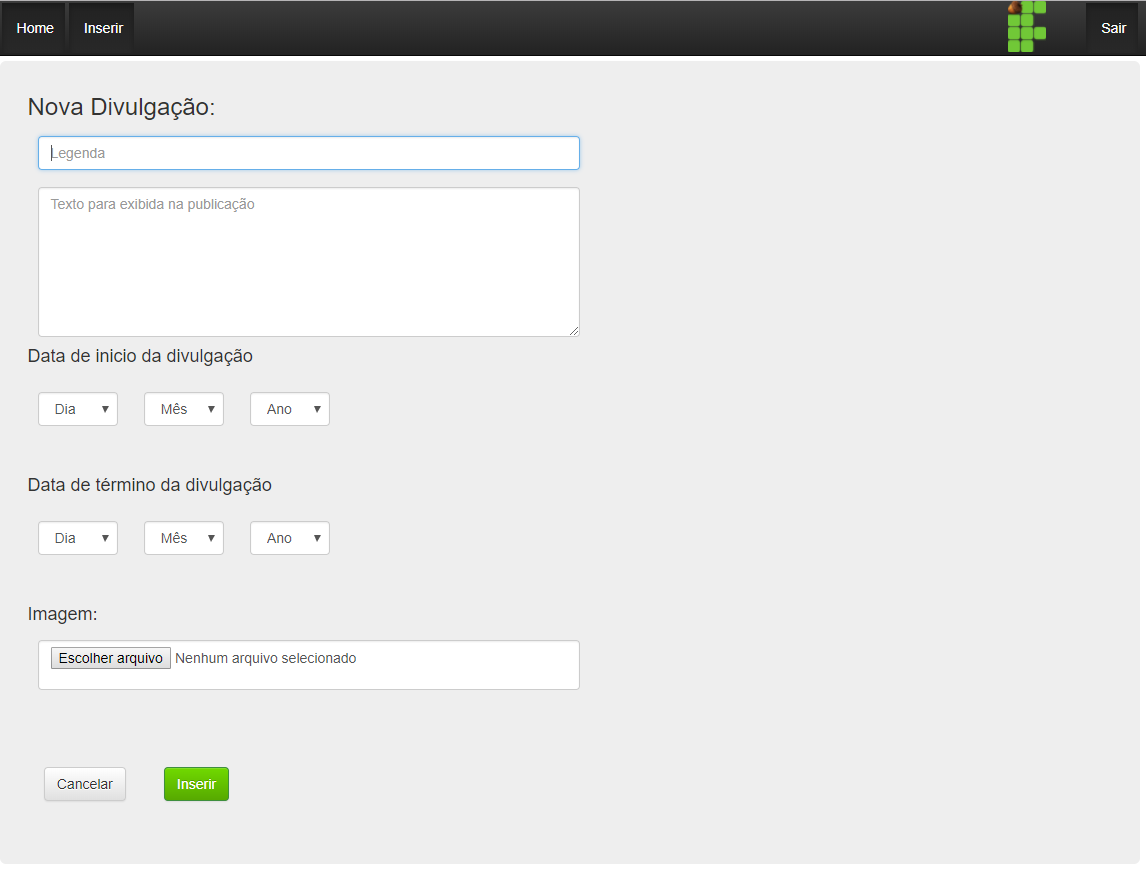
\includegraphics[scale=0.6]{figuras/administrador1}
\caption{Página de inserção no módulo administrador.}
\label{Rotulo}
\end{figure}

\section{Modulo Cliente}
\section{Modulo API}
\section{Arquitetura}
\section{Banco de Dados - Postgres}
\section{Possível solução para Implementação - Rapberry}
Desde a sua invenção em 1971, microprocessadores vem sendo usados no desenvolvimento dos mais variados tipos de eletrônicos ou outros equipamentos, substituindo até mesmo sistemas mecânicos. Algo que vai além de um simples software, os microprocessadores devem ser capazes controlar as ações de um dispositivo. \cite{rosenstark2007}

Para \cite{aristotelous2016}, o objetivo essencial de todos os tipos de empresa é a rentabilidade, podendo ela ser alcançada usando uma solução de baixo custo, boas tecnologias e com um preço atrativo. Teste do \cite{aristotelous2016} apresenta a possibilidade de se ter um servidor completamente funcional com sistema operacional Linux por um equipamento de 35\$, possibilitando a criação de um servidor, por exemplo de um repositório na nuvem com um baixo custo, flexibilidade e eficiência energética. 

Grandes servidores oferecem um melhor desempenho, entretanto, o baixo uso, a pouca eficiência energética ou até mesmo o pouco espaço podem limitar o uso desse tipo de equipamento. Nesse sentido, para \cite{Cusick}, placas de circuito oferecem vantagens como o uso de pouco espaço, desempenho significante com baixo custo e consumo, além do suporte a diversas soluções de software oferecendo múltiplas opções de interface com uma variante do Linux. 